
\begin{figure}[htbp]
\centering
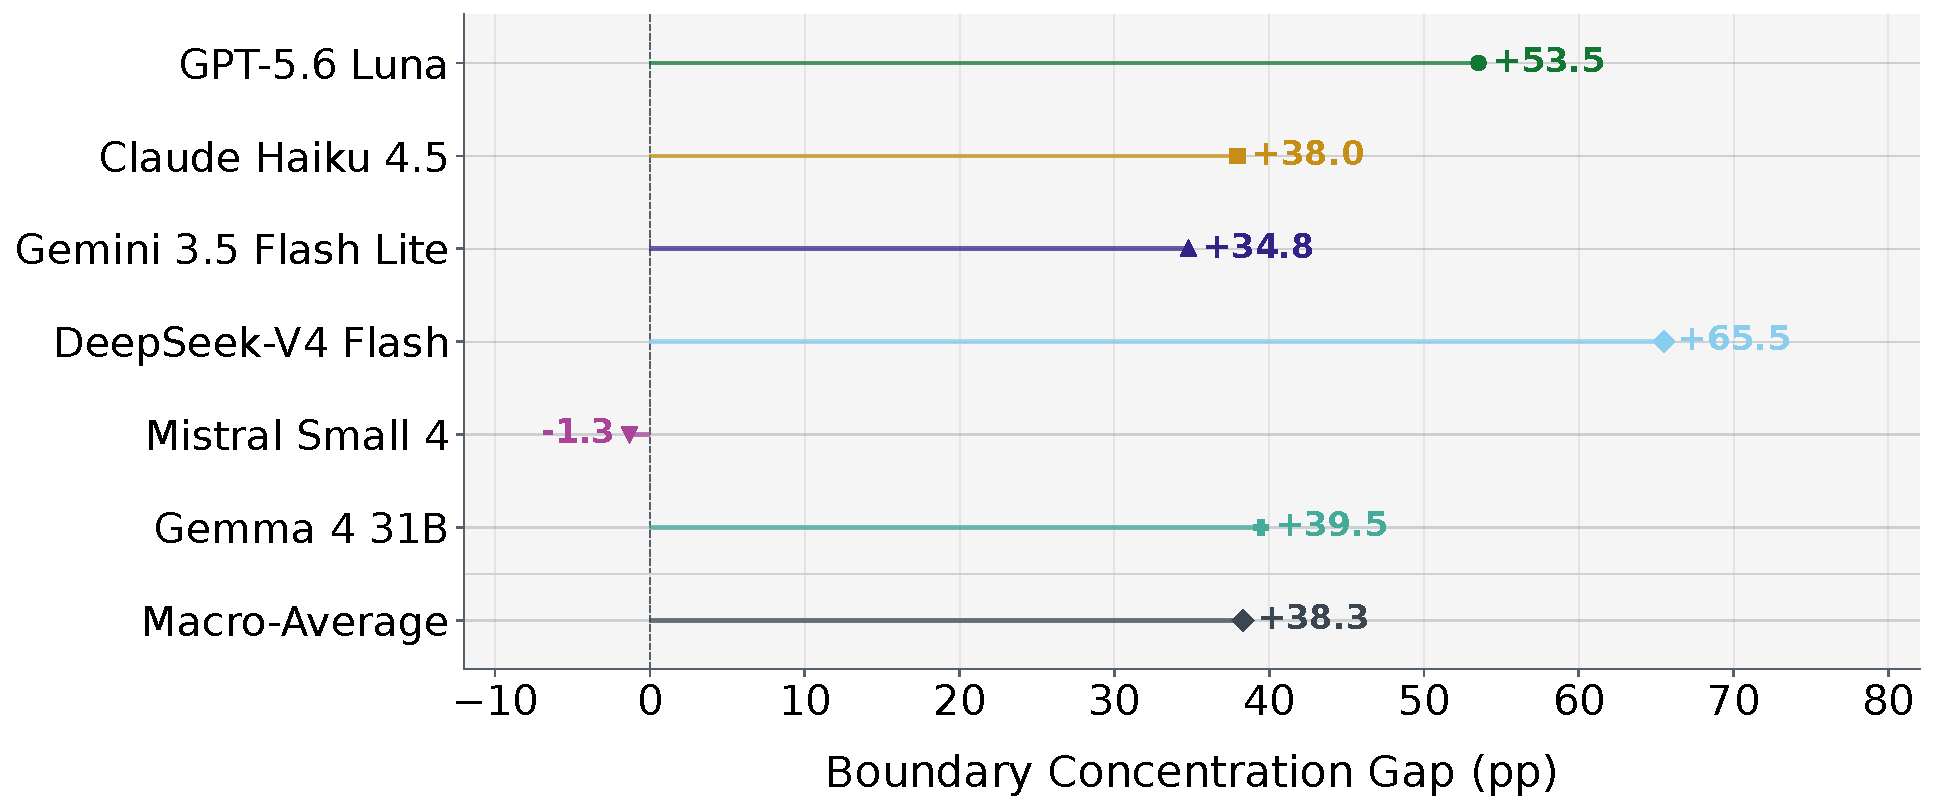
\includegraphics[width=0.8\textwidth]{joint/joint_boundary_gap.pdf}
\caption{\emph{Experiment 1} $\vert$ Boundary Share Gap by Model}
\label{fig:joint-boundary-gap}
\vspace{0.4em}
\begin{minipage}{\textwidth}
\footnotesize
\emph{Note.} The share of each ladder's full range spent at the statutory
boundary, refusal less grade level, from Table~\ref{tab:joint-shape}. A positive
value is a refusal ladder more concentrated at that one step than the reading
ladder is. Mistral Small 4 sits near zero at $-1.3$ points, being the one model
with no boundary effect to concentrate.
\end{minipage}
\end{figure}
